\documentclass[a4paper]{article}
\usepackage{ctex}
\usepackage[affil-it]{authblk}
\usepackage[backend=bibtex,style=numeric]{biblatex}
\usepackage{amsmath,amsthm,amssymb,amsfonts}
\usepackage{graphicx}
\usepackage{bm}

\usepackage{geometry}
\geometry{margin=1.5cm, vmargin={0pt,1cm}}
\setlength{\topmargin}{-1cm}
\setlength{\paperheight}{29.7cm}
\setlength{\textheight}{25.3cm}

\addbibresource{citation.bib}

\begin{document}
% =================================================
\title{微分方程数值解 2026 春夏作业四}

\author{曾申昊 3220100701
  \thanks{邮箱: \texttt{3097714673@qq.com}
                            \texttt{或} \texttt{3220100701@zju.edu.cn}}}
\affil{浙江大学}

\date{更新时间: \today}

\maketitle

% ============================================
\section*{Exercise 12.88}

\par 如图 \ref{fig:Exercise12-88} 所示，
这里仅绘制了最高阶数的稳定域。

\begin{figure}[ht]
    \centering
    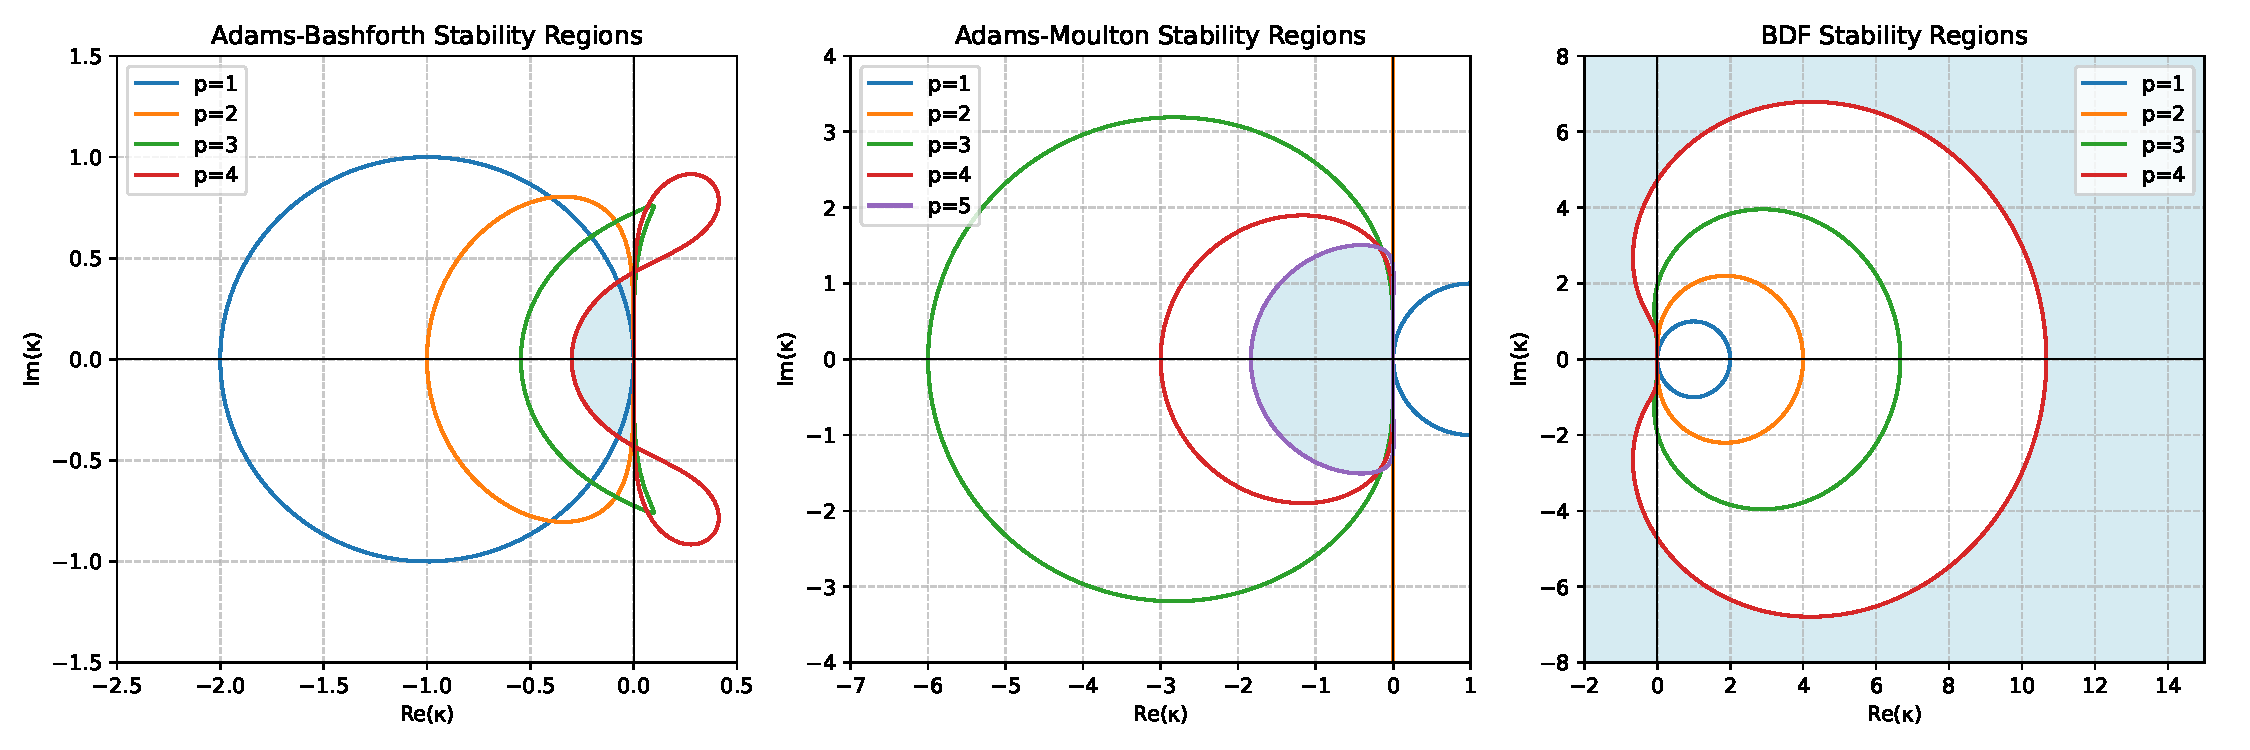
\includegraphics[width=0.9\textwidth]{figure/Exercise12-88.pdf}
    \vspace*{-2em}
    \caption{Exercise 12.88}
    \label{fig:Exercise12-88}
\end{figure}

\section*{Exercise 12.93}

\par $\theta_n$是方程 
$\theta_{n+s}+\displaystyle\sum_{i=0}^{s-1}\alpha_i\theta_{n+i}=0$ 的解，
满足初值
\begin{equation}
    \begin{bmatrix}
        \theta_0\\
        \theta_{-1}\\
        \vdots\\
        \theta_{-s+1}
    \end{bmatrix}
    =
    \begin{bmatrix}
        1\\
        0\\
        \vdots\\
        0
    \end{bmatrix}
\end{equation}
\par 需要求解非齐次方程 $y_{n+s}+\displaystyle\sum_{i=0}^{s-1}\alpha_iy_{n+i}=\psi_{n+s}$，
满足初值$y_0$，$y_{1}$，$\cdots$，$y_{s-1}$，并且有记号
\begin{equation}
    \begin{bmatrix}
        1 & \theta_1 & \theta_2 & \cdots & \theta_{s-2} & \theta_{s-1}\\
        0 & 1 & \theta_1 & \cdots & \theta_{s-3} & \theta_{s-2}\\
        0 & 0 & 1 & \cdots & \theta_{s-4} & \theta_{s-3}\\
        \vdots & \vdots & \vdots & \ddots & \vdots & \vdots\\
        0 & 0 & 0 & \cdots & 1 & \theta_1\\
        0 & 0 & 0 & \cdots & 0 & 1
    \end{bmatrix}
    \begin{bmatrix}
        \tilde{y}_{s-1}\\
        \tilde{y}_{s-2}\\
        \tilde{y}_{s-3}\\
        \vdots\\
        \tilde{y}_{1}\\
        \tilde{y}_{0}\\
    \end{bmatrix}
    =
    \begin{bmatrix}
        y_{s-1}\\
        y_{s-2}\\
        y_{s-3}\\
        \vdots\\
        y_{1}\\
        y_{0}\\
    \end{bmatrix}
\end{equation}

\begin{itemize}
    \item 当$n=0$时 
            \begin{equation}
                \begin{aligned}
                    y_s &= -\alpha_{s-1}y_{s-1} - \alpha_{s-2}y_{s-2} - \cdots - \alpha_0y_0 + \psi_{s}\\
                        &= -\alpha_{s-1}(\tilde{y}_{s-1}+\theta_1\tilde{y}_{s-2}+\cdots+\theta_{s-1}\tilde{y}_{0}) 
                        - \alpha_{s-2}(\tilde{y}_{s-2}+\theta_1\tilde{y}_{s-3}+\cdots+\theta_{s-2}\tilde{y}_{0}) - \cdots - \alpha_0
                        \tilde{y}_0 + \psi_{s}\\
                        &= -\alpha_{s-1}\tilde{y}_{s-1} - (\alpha_{s-1}\theta_1+\alpha_{s-2})\tilde{y}_{s-2} - \cdots -
                        (\alpha_{s-1}\theta_{s-1}+\alpha_{s-2}\theta_{s-2}+\cdots+\alpha_{0})\tilde{y}_0 + \psi_{s}\\
                        &= \theta_1\tilde{y}_{s-1} +\theta_2\tilde{y}_{s-2} + \cdots +
                        \theta_s\tilde{y}_0 + \psi_{s}\\
                \end{aligned}
            \end{equation}
            符合通解公式 $y_n=\displaystyle
            \sum_{i=0}^{s-1} \theta_{n-i} \tilde{y}_{i} + \displaystyle\sum_{i=s}^{n}\theta_{n-i}\psi_i$
    \item 设$n=k-1$时上式同样成立
    \item 则当$n=k$时
            \begin{equation}
                \begin{aligned}
                    y_{k+s} &= -\sum_{i=0}^{s-1}\alpha_i y_{k+i} +\psi_{k+s}\\
                    &=-\sum_{i=0}^{s-1}\alpha_i \left(\sum_{j=0}^{s-1} \theta_{k+i-j}\tilde{
                        y}_j + \sum_{j=s}^{k+i}\theta_{k+i-j}\psi_j\right) + \psi_{k+s}\\
                    &=-\sum_{i=0}^{s-1}\alpha_i \left(\sum_{j=0}^{s-1} \theta_{k+i-j}\tilde{
                        y}_j\right) - \sum_{i=0}^{s-1}\alpha_i \left(\sum_{j=s}^{k+i}\theta_{k+i-j}\psi_j\right) + \psi_{k+s}\\
                    &=-\sum_{j=0}^{s-1} \tilde{y}_j\left(\sum_{i=0}^{s-1} \alpha_i\theta_{k+i-j}\right) 
                        - \sum_{j=s}^{k+s-1} \psi_j\left(\sum_{i=0}^{s-1}\alpha_i\theta_{k+i-j}\right) + \psi_{k+s}\\
                    &=\sum_{j=0}^{s-1} \theta_{k+s-j}\tilde{y}_j + \sum_{j=s}^{k+s-1} \theta_{k+s-j}\psi_j + \psi_{k+s}\\
                    &=\sum_{j=0}^{s-1} \theta_{k+s-j}\tilde{y}_j + \sum_{j=s}^{k+s} \theta_{k+s-j}\psi_j
                \end{aligned}
            \end{equation}
\end{itemize}

\section*{Exercise 12.98}

\par 利用反证法，假设该LMM是不相容的，
即下面两个条件有一个不成立：
\begin{equation}
    \sum_{j=0}^{s}\alpha_j=0
    \qquad
    \sum_{j=0}^{s} j\alpha_j = \sum_{j=0}^{s} \beta_j
\end{equation}
\par 假设前者不成立$\displaystyle\sum_{j=0}^{s}\alpha_j\neq0$，考虑初值问题
\begin{equation}
    u'(t)=0 \qquad u(0)=1
\end{equation}
\par 其精确解为$u(t)=1$，由收敛性可得
对任意固定的$T=Nk$，当$k\to0$时，数值解$U^N\to u(T)=1$，又由于LMM的定义式为
\begin{equation}
    \sum_{j=0}^{s}\alpha_j U^{n+j} = k\sum_{j=0}^{s} \beta_j f(U^{N+j},t_{n+j})=0
\end{equation}
\par 两边取极限可得$\displaystyle\sum_{j=0}^{s}\alpha_j=0$，产生矛盾。

\par 假设后者不成立$\displaystyle\sum_{j=0}^{s}j\alpha_j\neq \sum_{j=0}^{s} \beta_j$，考虑初值问题
\begin{equation}
    u'(t)=1 \qquad u(0)=0
\end{equation}
\par 其精确解为$u(t)=t$，由LMM的定义式得
\begin{equation}
    \sum_{j=0}^{s}\alpha_j U^{n+j} = k\sum_{j=0}^{s} \beta_j f(U^{N+j},t_{n+j})=
    k\sum_{j=0}^{s} \beta_j
\end{equation}
\par 由收敛性可得
当$k\to0$时，$U^{n+j}\to u(T+jk)=T+jk$，
两边除以$k$后取极限可得$\displaystyle\sum_{j=0}^{s}j\alpha_j = \sum_{j=0}^{s} \beta_j$，产生矛盾。


% ===============================================

\printbibliography

\end{document}